\documentclass{article}

% PACKAGES for math, diagrams, and layout
\usepackage{amsmath}
\usepackage{amssymb}
\usepackage{tikz}
\usepackage{geometry}
\usepackage{graphicx} % Good practice to include for graphics

% DOCUMENT LAYOUT
\geometry{a4paper, margin=1in}

% --- DOCUMENT START ---
\begin{document}

\title{Two-Source Interference of Sound and Light Waves}
\author{Concise Notes \& Competition Problems}
\date{}
\maketitle

\section{The Core Principle: Superposition \& Coherence}

When two or more waves meet at a point, the resultant displacement is the vector sum of the individual displacements. This is the \textbf{principle of superposition}.

For interference to be observed, the sources must be \textbf{coherent}. This means they emit waves with a \textbf{constant phase difference} and the same frequency.

\begin{itemize}
    \item \textbf{Constructive Interference:} Waves arrive \textbf{in phase}. Crests meet crests. This results in a \textbf{maximum} amplitude (bright fringe for light, loud sound for audio).
    \item \textbf{Destructive Interference:} Waves arrive \textbf{out of phase} (by $180^\circ$ or $\pi$ radians). Crests meet troughs. This results in a \textbf{minimum} or zero amplitude (dark fringe for light, quiet spot for sound).
\end{itemize}

\begin{center}
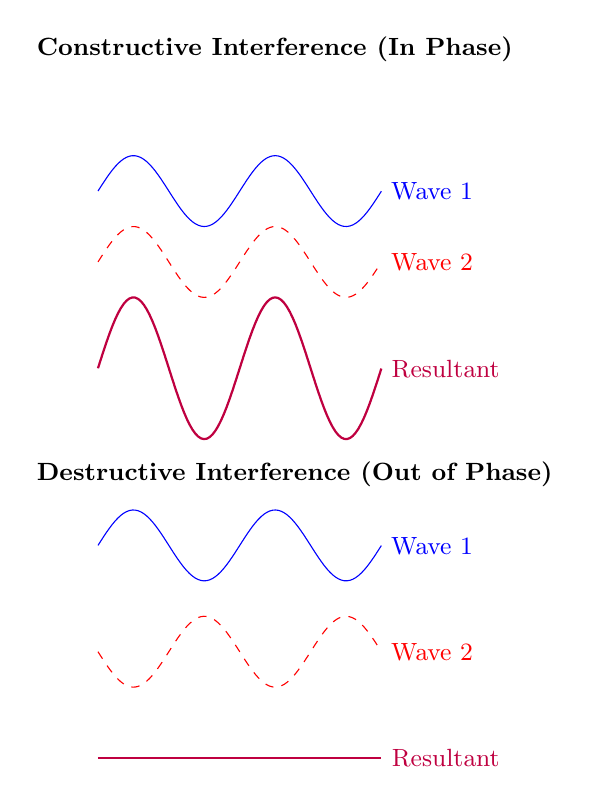
\begin{tikzpicture}[scale=0.9, every node/.style={font=\small}]
    % --- Constructive Interference ---
    \node[anchor=west] at (-1, 3) {\textbf{Constructive Interference (In Phase)}};
    \draw[blue, domain=0:4, samples=100] plot (\x, {1 + 0.5*sin(180*\x)}) node[right] {Wave 1};
    \draw[red, dashed, domain=0:4, samples=100] plot (\x, {0 + 0.5*sin(180*\x)}) node[right] {Wave 2};
    \draw[purple, thick, domain=0:4, samples=100] plot (\x, {-1.5 + 1*sin(180*\x)}) node[right] {Resultant};

    % --- Destructive Interference (CORRECTED) ---
    \node[anchor=west] at (-1, -3) {\textbf{Destructive Interference (Out of Phase)}};
    \draw[blue, domain=0:4, samples=100] plot (\x, {-4 + 0.5*sin(180*\x)}) node[right] {Wave 1};
    \draw[red, dashed, domain=0:4, samples=100] plot (\x, {-5.5 - 0.5*sin(180*\x)}) node[right] {Wave 2};
    \draw[purple, thick] (0,-7) -- (4,-7) node[right] {Resultant};
\end{tikzpicture}
\end{center}

\hrulefill

\section{Path Difference: The Key to Interference}

The type of interference at a point depends on the \textbf{path difference} ($\Delta L$), which is the difference in the distance traveled by the two waves from their sources to that point. The path difference creates a \textbf{phase difference} ($\Delta \phi$). The relationship is:
\[ \Delta \phi = \frac{2\pi}{\lambda} \Delta L \]
\subsection*{Conditions for Interference}
\begin{itemize}
    \item \textbf{Constructive Interference (Maxima):} $\Delta L = n\lambda \quad \text{where } n = 0, 1, 2, ...$
    \item \textbf{Destructive Interference (Minima):} $\Delta L = \left(n + \frac{1}{2}\right)\lambda \quad \text{where } n = 0, 1, 2, ...$
\end{itemize}

\hrulefill

\section{Advanced Topics \& Problem-Solving Techniques}

\subsection{The Small Angle Approximation}
In many setups, the screen distance $l$ is much larger than the slit separation $d$ ($l \gg d$). For small angles $\theta$, we can approximate: $\sin\theta \approx \tan\theta = y/l$.
The path difference becomes: $\Delta L = d \sin \theta \approx \frac{dy}{l}$. This allows us to find the fringe spacing $\Delta y = \frac{\lambda l}{d}$.

\subsection{Intensity Distribution}
If two coherent sources each have intensity $I_0$, the resultant intensity $I$ at a point with phase difference $\phi$ is:
\[ I = 4I_0 \cos^2\left(\frac{\phi}{2}\right) = 4I_0 \cos^2\left(\frac{\pi d \sin\theta}{\lambda}\right) \]
The \textbf{maximum intensity} is $I_{max} = 4I_0$.

\subsection{Interference with Non-Normal Incidence}
If the incoming light arrives at an angle $\alpha$ and leaves at an angle $\beta$.
\begin{itemize}
    \item \textbf{Case 1 (Opposite Sides):} If the angles are on opposite sides of the normal, the path differences add up: $\Delta L = d \sin\alpha + d \sin\beta$.
    \item \textbf{Case 2 (Same Side):} If the angles are on the same side of the normal, the path differences subtract: $\Delta L = |d \sin\alpha - d \sin\beta|$.
\end{itemize}

\subsection{Interference by Reflection}
Reflection from a denser medium causes a $\boldsymbol{\pi}$ \textbf{radian ($180^\circ$) phase shift}, which is equivalent to adding $\lambda/2$ to the path length. This swaps the conditions for constructive and destructive interference.

\hrulefill
\newpage

\section*{Olympiad Problems with Solutions}

\subsection{Problem 1 (SPhO 2024)}
\begin{quote}
Figure 10 shows an opaque screen in which there are two narrow parallel slits, P and Q, separated by a distance $d$. A beam of monochromatic light of wavelength $\lambda$ is incident on the screen at an angle $\alpha$ to the normal. Consider light emerging from the slits at an angle $\beta$ to the normal. Find an expression for the total path difference between rays 1 and 2 as a result of passing through the slits. Hence find the condition for the light emerging at angle $\beta$ to be of maximum intensity.
\end{quote}
\begin{center}
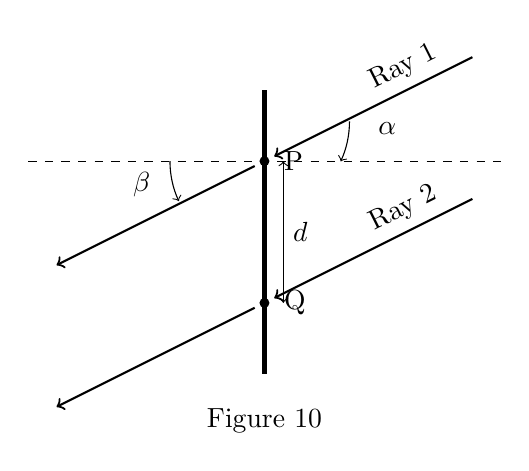
\begin{tikzpicture}[scale=1.2]
    % Slit screen
    \draw[ultra thick] (0,-1.5) -- (0,1.5);
    \node at (0,0.75) [label=right:P] (P) {};
    \node at (0,-0.75) [label=right:Q] (Q) {};
    \fill (P) circle (1.5pt);
    \fill (Q) circle (1.5pt);
    \draw[<->] (0.2,0.75) -- (0.2,-0.75) node[midway, right] {$d$};

    % Normal line at P
    \draw[dashed] (-2.5,0.75) -- (2.5,0.75);

    % Incoming rays from top-right
    \coordinate (ray1_start) at (2.2, 1.85);
    \draw[->, thick] (ray1_start) -- (P) node[pos=0.3, above, sloped] {Ray 1};
    \coordinate (ray2_start) at (2.2, 0.35);
    \draw[->, thick] (ray2_start) -- (Q) node[pos=0.3, above, sloped] {Ray 2};

    % Outgoing rays to bottom-left
    \coordinate (ray1_end) at (-2.2, -0.35);
    \draw[->, thick] (P) -- (ray1_end);
    \coordinate (ray2_end) at (-2.2, -1.85);
    \draw[->, thick] (Q) -- (ray2_end);

    % Angle alpha
    \draw[->] (0.9, 1.17) arc(0:-25:1.0);
    \node at (1.3, 1.1) {$\alpha$};

    % Angle beta
    \draw[->] (-1.0, 0.75) arc(180:205:1.0);
    \node at (-1.3, 0.5) {$\beta$};

    \node at (0,-2) {Figure 10};
\end{tikzpicture}
\end{center}
\paragraph{Solution:}
\begin{enumerate}
    \item \textbf{Path difference before slits ($\Delta L_1$):} As shown in the corrected diagram, the incoming beam from the top-right means Ray 1 travels a longer path than Ray 2 to reach the slits. This extra distance is $d \sin \alpha$.
    \item \textbf{Path difference after slits ($\Delta L_2$):} The rays emerge and travel to the bottom-left, on the opposite side of the normal. In this direction, Ray 2 travels a longer path than Ray 1. This extra distance is $d \sin \beta$.
    \item \textbf{Total path difference ($\Delta L_{\text{total}}$):} Since the rays are on opposite sides of the normal, the total path difference is the \textbf{sum} of the two individual path differences.
    \[ \Delta L_{\text{total}} = d \sin \alpha + d \sin \beta = d(\sin \alpha + \sin \beta) \]
    \item \textbf{Condition for maximum intensity:} For constructive interference (maximum intensity), the total path difference must be an integer multiple of the wavelength $\lambda$.
    \[ d(\sin \alpha + \sin \beta) = n\lambda, \quad \text{where } n = 0, 1, 2, ... \]
\end{enumerate}

\hrulefill

\subsection{Problem 2 (SPhO 2023) \& 4 (SPhO 2019)}
\begin{quote}
A sound source S and a detector D are placed 120 m apart. A reflector is parallel to the line SD. At position 1 (90 m from SD), the direct and reflected waves are in phase. The reflector is moved away to position 2.
\begin{itemize}
    \item \textbf{2023 Problem:} At position 2, intensity is zero for the first time. Find $h$.
    \item \textbf{2019 Problem:} At position 2, intensity is maximum again for the first time. Find $h$.
\end{itemize}
\end{quote}
\begin{center}
\begin{tikzpicture}
    \node at (0,0) [circle,fill,inner sep=1pt,label=above:S] {};
    \node at (8,0) [circle,fill,inner sep=1pt,label=above:D] {};
    \draw[<->] (0,-0.2) -- (8,-0.2) node[midway, below] {120 m};
    % Reflector
    \draw[thick] (0,3) -- (8,3) node[midway, label={[label distance=0.1cm]90:Reflector}] {};
    \node at (9,3) {Position 1};
    \draw[thick, dashed] (0,4) -- (8,4);
    \node at (9,4) {Position 2};
    % Distances
    \draw[<->] (9.5,3) -- (9.5,4) node[midway, right] {$h$};
    \draw[<->] (8.2,0) -- (8.2,3) node[midway, right] {90 m};
\end{tikzpicture}
\end{center}
\paragraph{Solution:} ($\lambda=1.33$ m)
Let $L=120$ m and $y$ be the reflector distance. Path difference $\Delta L_{geo} = 2 \sqrt{y^2 + (L/2)^2} - L$.
\begin{enumerate}
    \item \textbf{Condition at Position 1:} At $y_1 = 90$ m, waves are in phase (constructive). With a $\pi$ phase shift on reflection, the condition is $\Delta L_{geo} = (m+1/2)\lambda$.
    $\Delta L_1 = 2 \sqrt{90^2 + 60^2} - 120 = 96.33$ m.
    $m + 1/2 = 96.33/1.33 = 72.43 \implies m=72$.
    \item \textbf{For SPhO 2023 (First Minimum):} The next fringe is destructive ($\Delta L_{geo} = k\lambda$) at order $k=73$.
    $\Delta L_2 = 73 \times 1.33 = 97.09$ m.
    $2 \sqrt{y_2^2 + 60^2} - 120 = 97.09 \implies y_2 = 90.45$ m. Thus, $h = \textbf{0.45 m}$.
    \item \textbf{For SPhO 2019 (Next Maximum):} The next fringe is constructive ($\Delta L_{geo} = (m'+1/2)\lambda$) at order $m'=73$.
    $\Delta L_2 = (73.5)\lambda = 97.755$ m.
    $2 \sqrt{y_2^2 + 60^2} - 120 = 97.755 \implies y_2 = 90.85$ m. Thus, $h = \textbf{0.85 m}$.
\end{enumerate}

\hrulefill

\subsection{Problem 3 (SPhO 2021)}
\begin{quote}
Consider Young's double slit experiment. (a) Under what condition does it show an interference pattern? (b) Determine the conditions for constructive and destructive interference. (c) Determine the distance $\Delta y$ between adjacent fringes, assuming $\theta$ is small. (d) Determine the intensity I of the diffraction pattern's maxima.
\end{quote}
\paragraph{Solution:}
(a) The light from the two slits must be \textbf{coherent}. (b) Path difference is $\Delta L = d \sin \theta$. For constructive, $d \sin \theta = n\lambda$. For destructive, $d \sin \theta = (n+1/2)\lambda$. (c) Using small angle approx, $\sin\theta \approx y/l$. The fringe spacing is $\Delta y = \frac{\lambda l}{d}$. (d) Intensity is $I = 4I_0 \cos^2(\phi/2)$. The maximum intensity $I_{max}$ is $\textbf{4I}_0$.

\newpage
\section*{New Challenge Problems with Solutions}

\subsection{Problem 1: The Tilted Screen}
\begin{quote}
In a Young's double-slit experiment, two slits separated by $d=0.20$ mm are illuminated by a laser of wavelength $\lambda = 500$ nm. The screen is placed a distance $l=1.0$ m away, but it is tilted at an angle $\gamma=15^\circ$ with respect to the standard y-axis. Find the distance along the screen from the central maximum to the first bright fringe.
\end{quote}
\paragraph{Solution:}
The path difference to a point on the screen is $\Delta L = d\sin\theta$. For the first bright fringe ($n=1$), $\Delta L = \lambda$.
\[ \sin\theta = \frac{\lambda}{d} = \frac{500 \times 10^{-9} \text{ m}}{0.20 \times 10^{-3} \text{ m}} = 0.0025 \]
Using the small angle approximation, $\tan\theta \approx \sin\theta = 0.0025$. The vertical position on a normal screen would be $y = l\tan\theta = (1.0 \text{ m})(0.0025) = 2.5$ mm. On the tilted screen, this vertical distance $y$ relates to the on-screen distance $z$ by $y = z \cos\gamma$.
\[ z = \frac{y}{\cos\gamma} = \frac{2.5 \text{ mm}}{\cos(15^\circ)} = \frac{2.5 \text{ mm}}{0.9659} = \textbf{2.59 mm} \]

\hrulefill

\subsection{Problem 2: The Coated Mirror}
\begin{quote}
A microwave transmitter T is placed a distance $h=5.0$ cm above a large, flat metal plate. A receiver R is placed a horizontal distance $L=20.0$ cm away, also at height $h$. The plate is coated with a thin layer of plastic ($n_p=1.50$) of thickness $t=1.0$ cm. The microwaves have a wavelength of $\lambda=4.0$ cm. Is the interference at the receiver R constructive, destructive, or intermediate?
\end{quote}
\paragraph{Solution:}
The geometric path difference is $\Delta L_{geo} = L_{refl} - L_{direct}$.
$L_{refl} = 2\sqrt{(L/2)^2 + h^2} = 2\sqrt{(10.0)^2 + (5.0)^2} = 22.36$ cm.
$\Delta L_{geo} = 22.36 - 20.0 = 2.36$ cm.
The wave reflects from the metal plate, which is a denser medium, so it undergoes a $\pi$ phase shift. This is equivalent to adding $\lambda/2$ to the path difference.
\[ \Delta L_{eff} = \Delta L_{geo} + \frac{\lambda}{2} = 2.36 \text{ cm} + \frac{4.0 \text{ cm}}{2} = 4.36 \text{ cm} \]
To determine the type of interference, we compare this to the wavelength:
\[ \frac{\Delta L_{eff}}{\lambda} = \frac{4.36 \text{ cm}}{4.0 \text{ cm}} = 1.09 \]
Since this value is very close to an integer ($n=1$), the interference is nearly \textbf{constructive}.

\hrulefill

\subsection{Problem 3: Three-Slit Interference}
\begin{quote}
Three identical and coherent sources, $S_1$, $S_2$, and $S_3$, are equally spaced by a distance $d$. (a) Find the phase difference, $\phi$, between adjacent sources at an angle $\theta$. (b) Using phasors, find the resultant intensity $I$ in terms of $I_0$. (c) What is the intensity of the principal maxima? (d) What is the condition for the first minimum?
\end{quote}
\paragraph{Solution:}
(a) The phase difference between adjacent sources is $\phi = \frac{2\pi d \sin\theta}{\lambda}$.
(b) The resultant amplitude $A$ is the sum of three phasors with phases $0, \phi, 2\phi$. The sum is $A = E_0(1+\cos\phi+\cos(2\phi)) + iE_0(\sin\phi+\sin(2\phi))$. The intensity $I \propto A^2$ simplifies to $I = I_0(1 + 2\cos\phi)^2$.
(c) Principal maxima occur when $\phi=2\pi n$, so $\cos\phi=1$. The intensity is $I_{max} = I_0(1+2)^2 = \textbf{9I}_0$. This occurs when $d\sin\theta = n\lambda$.
(d) The first minimum (zero intensity) occurs when the three phasors form a closed triangle, which happens when $\phi = 2\pi/3$. This gives the condition $d\sin\theta = \frac{\lambda}{3}$.

\end{document}
% --- DOCUMENT END ---